\documentclass[10pt,a4paper]{beamer}
\usepackage[utf8]{inputenc}
\usepackage[english]{babel}
\usepackage{amsmath}
\usepackage{amsfonts}
\usepackage{amssymb}
\usepackage{listings}
\usepackage{hyperref}
\usepackage{graphicx}
\usepackage{listings}
\usepackage{mathpartir}
\hypersetup{colorlinks,urlcolor=blue}

\usetheme{Warsaw}

\lstset
{
	basicstyle = \ttfamily\tiny,
	breaklines = true,
	frame = single
}

\begin{document}

\author[Di Giacomo et al.]
{Francesco ~Di Giacomo \inst{1} \\
	\and Mohamed ~Abbadi \inst{1} \\
	\and Agostino ~Cortesi \inst{1} \\
	\and Pieter ~Spronck \inst{2} \\
	\and Giuseppe ~Maggiore \inst{3}}
\institute[Universities Here and There] % (optional)
{
  Università Ca' Foscari di Venezia
  \and Tilburg University
  \and Hogeschool Rotterdam
}
\date{}
\title{Build game scripts DSL's with the Metacasanova metacompiler}

\frame{\titlepage}

\begin{frame}
\frametitle{Reasons behind scripting DSL's}
Games contain very complex behaviours:
\begin{itemize}
\item Wait to be close enough to interact with an item.
\item Perform an action only if the key was pressed and then released.
\item Execute two tasks in parallel and take the result of the one that terminates first.
\item Prioritized behaviours.
\end{itemize}
\end{frame}

\begin{frame}
	\frametitle{Reasons behind scripting DSL's}
	\framesubtitle{Examples}
	Games contain very complex behaviours:
	\begin{itemize}
		\item Interacting with a door only if you are close to it.
		\item Shoot with a handgun
		\item A special moves in a fighting game: we want that pressing a key in the combination is done within a given time.
		\item A guard AI that patrols with lowest priority, shoot the enemy with medium priority, and take cover with highest priority.
	\end{itemize}
\end{frame}

\begin{frame}
	\frametitle{Reasons behind scripting DSL's}
	\framesubtitle{Advantages of a DSL}
	\begin{itemize}
		\item These behaviours are hard to express in GPL's because they require constructs not provided within the language.
		\item Wait for a certain amount of time, wait for a condition, concurrency operators, priority operators, ...
		\item We would really like to be able to write \texttt{wait 5.0f} in our code.
	\end{itemize}
\end{frame}

\begin{frame}
	\frametitle{Implementing DSL's for games}
	\begin{itemize}
		\item Possible hard-coded solutions: strategy pattern, monadic coroutines, generators (virtuality involved).
		\item State machines, compiler for a custom scripting DSL's (better performance).
		\item It is possible to create a multi-threaded game engine, but impossible to create a thread to handle each one of the situations above.
	\end{itemize}
\end{frame}

\begin{frame}
	\frametitle{Compilers are a very popular choice}
	\begin{itemize}
		\item Warcraft III: Just Another Script Syntax (JASS)
		\item Starcraft II: Galaxy Script
		\item ArmA series: Status Quo Scripts (SQF).
		\item Neverwinter Nights: NWN Script.
		\item Unreal Engine: UnrealScript.
	\end{itemize}
	
	\begin{figure}
		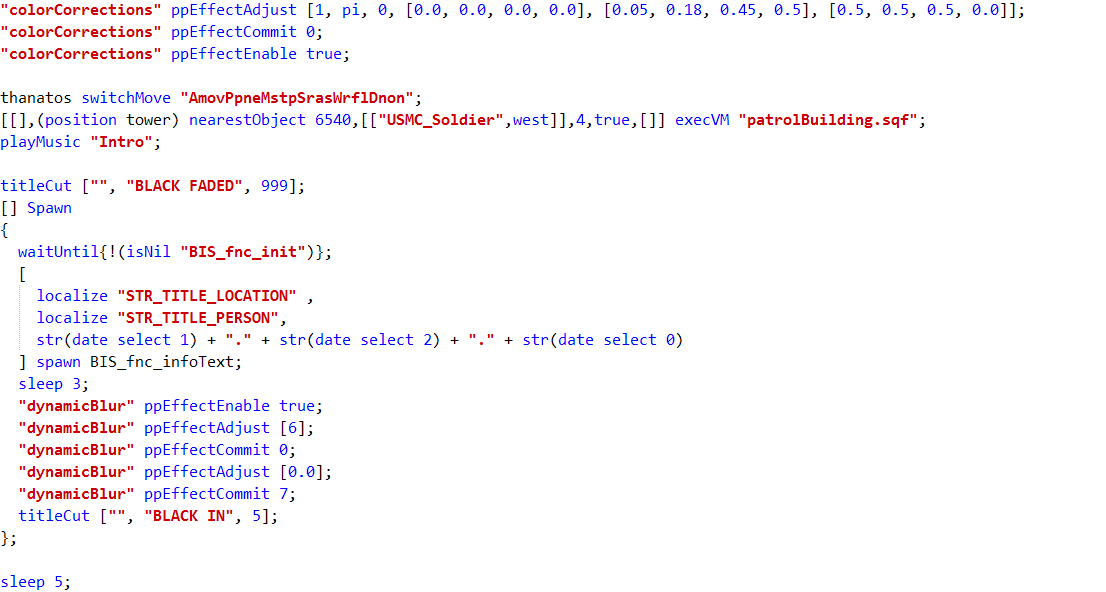
\includegraphics[scale = 0.25]{Pictures/sqf}
		\caption{Code snippet from SQF script}
	\end{figure}
\end{frame}

\begin{frame}
	\frametitle{Compilers are complex}
	\begin{itemize}
		\item Compilers are very complex pieces of software.
		\item Parser, Type checker, intermediate code generation, interpreter or assembler.
		\item Expensive, hard to add extra features to the language.
	\end{itemize}
\end{frame}

\begin{frame}
	\frametitle{Compilers are repetitive}
	\begin{enumerate}
		\item Write a formalism for the grammar of the language.
		\item Build a parser for the syntax analysis based on the grammar.
		\item Write a formalism for the type system.
		\item Build a type checker for the type analysis based on the type system.
		\item Write the semantics of the language
		\item Generate code according to the semantics.
	\end{enumerate}
\end{frame}

\begin{frame}
	\frametitle{Compilers are repetitive}
	\begin{itemize}
		\item The only ``creative'' part of the process is step 1,3,5 (on the paper)
		\item The rest is just about implementing those points in the chosen language.
		\item What if it was possible to have a compiler that accepts as input a language definition, a program written in that language, and outputs executable code?
	\end{itemize}
\end{frame}

\begin{frame}
	\frametitle{Idea behind Metacasanova}
	\begin{itemize}
		\item Write the language definition (type system and semantics) as a real program.
		\item Generate code according to this definition.
		\item Advantage: no need to encode the definition in a programming language (no hard-coded compiler).
	\end{itemize}
\end{frame}

\begin{frame}
	\frametitle{Overview of Metacasanova}
	\begin{itemize}
		\item \textbf{Data declaration}: used to represent the syntactical constructs of the language (meta-data).
		\item \textbf{Function declaration}: They define the meta-types (meta-types transformations).
		\item \textbf{Rules}: They define how the semantics of the syntactical constructs (language semantics)
		\item \textbf{Subtyping}: They define equivalence among meta-types
	\end{itemize}
\end{frame}

\begin{frame}[fragile]
	\frametitle{Examples}
	
	\textbf{Data declarations:}
	\begin{lstlisting}
Data Expr -> "+" -> Expr : Expr  Priority 500
Data "$f" -> <<float>> : Value Priority 10000
	\end{lstlisting}
	
	\textbf{Function declarations:}
	\begin{lstlisting}
Func "eval" -> Expr : Evaluator => Value
	\end{lstlisting}
	
	\textbf{Rules:}
	\begin{lstlisting}
eval a => $f c
eval b => $f d
<<c + d>> => res
-----------------------------
eval (a + b) => $f res
	
------------------------
eval ($f f) => $f f
	\end{lstlisting}
	
	\textbf{Subtyping:}
	\begin{lstlisting}
Value is Expr
	\end{lstlisting}
\end{frame}

\begin{frame}
	\frametitle{Case study: Casanova 2.5}
	\framesubtitle{Elements of the language}
	
	\begin{itemize}
		\item \textbf{Entities:} They contain both the data and the behaviour of the objects in the game
		\item \textbf{Rules:} They define the behaviour of the entity. Once a rule ends its execution it is restarted at the next frame.
		\item \textbf{Domain:} A set of entity attributes the rule is allowed to change. A rule can always read all fields but can modify only those in the domain through a \texttt{yield} statement.
	\end{itemize}
\end{frame}

\begin{frame}[fragile]
	\frametitle{Example of program in Casanova}
	\begin{lstlisting}[basicstyle = \ttfamily\small]
entity Guard = {
Position  : Vector2
Velocity  : Vector2

rule Position = Position + Velocity * dt
	
rule Velocity =
	wait Position.X >= 300f || Position.X <= 0f
	yield new Vector2(-Velocity.X, 0f)
}
	\end{lstlisting}
\end{frame}

\begin{frame}
	\frametitle{Rule pausing}
	Rule execution can be paused with built-in statements:
	\begin{itemize}
		\item \texttt{wait} takes either a floating point value or a predicate. In the first version the rule is paused by the given amount of seconds, in the second it is paused until the condition is met.
		\item \texttt{yield} updates the fields in the domain with the given values. The rule execution is paused by one frame in order to be able to see the changes at the next game update.
	\end{itemize}
\end{frame}

\begin{frame}
	\frametitle{Semantics of wait}
	\begin{mathpar}
		\small
		\inferrule
		{\langle t - dt > 0 \rangle \; \Rightarrow \; \texttt{true}}
		{\langle \mathtt{wait} \; t;k \; dt \rangle \; \Rightarrow \; \langle \mathtt{wait} \; t - dt ; k \; dt \rangle}
		
		\inferrule
		{\langle t - dt > 0 \rangle \; \Rightarrow \; \texttt{false}}
		{\langle \mathtt{wait} \; t ; k \; dt \rangle \; \Rightarrow \; \langle k \; dt \rangle}
		
		\small
		\inferrule
		{\langle c \rangle \; \Rightarrow \; \mathtt{true}}
		{\langle \mathtt{wait} \; c;k \; dt \rangle \; \Rightarrow \; \langle k \; dt\rangle}
		
		\inferrule
		{\langle c \rangle \; \Rightarrow \; \mathtt{false}}
		{\langle \mathtt{wait} \; c;k \; dt \rangle \; \Rightarrow \; \langle \mathtt{wait} \; c;k \; dt \rangle}
	\end{mathpar}
\end{frame}

\begin{frame}[fragile]
	\frametitle{Implementation of wait in Metacasanova}
	In the following waiting on a condition is called \texttt{when} because Metacasanova does not currently support operators overloading
	\begin{lstlisting}
eval expr ctxt => ($f t)
<<t <= dt>> == false
----------------------------------
eval_s (wait expr) k ctxt dt => Suspend (wait $f (<<t - dt>>));k ctxt

eval expr ctxt => ($f t)
<<t <= dt>> == true
----------------------------------
eval_s (wait expr) k ctxt dt => Resume k ctxt


eval expr ctxt => ($b true)
---------------------------------------------
eval_s (when expr) k ctxt dt => Atomic k ctxt

eval expr ctxt => ($b false)
------------------------------------------
eval_s (when expr) k ctxt dt => Suspend (when expr);k ctxt
	\end{lstlisting}
	
\end{frame}

\begin{frame}
	\frametitle{Results: patrol script}
	\begin{itemize}
		\item Script making a guard patrol two checkpoints
		\item Tests run with the script written in Casanova 2.5 and Python.
		\item Python is used as a scripting language is several games (e.g. World in Conflict, Civilization IV).
		\item We neglected C\# because we already have benchmarks for that in Casanova 2.0 and they are faster of several orders of magnitude.
	\end{itemize}
\end{frame}

\begin{frame}
	\frametitle{Results: patrol script}
	\begin{table}
		\centering
		\tiny	
		\begin{tabular}{|c|c|c|}
			\hline
			\multicolumn{3}{|c|}{\textbf{Casanova 2.5}} \\
			\hline
			Entity \# & Average update time (ms) & Frame rate \\
			\hline
			100 & 0.00349 & 286.53 \\
			\hline
			250 & 0.00911 & 109.77 \\
			\hline
			500 & 0.01716 & 58.275 \\
			\hline
			750 & 0.02597 & 38.506 \\
			\hline
			1000 & 0.03527 & 28.353 \\
			\hline
			\multicolumn{3}{|c|}{\textbf{Python}} \\
			\hline
			Entity \# & Average update time (ms) & Frame rate \\
			\hline
			100 & 0.00132 & 756.37 \\
			\hline
			250 & 0.00342 & 292.05 \\
			\hline
			500 & 0.00678 & 147.54 \\
			\hline
			750 & 0.01087 & 91.988 \\
			\hline
			1000 & 0.01408 & 71.002 \\
			\hline
		\end{tabular}
		\quad
		\begin{tabular}{|c|c|}
			\hline
			\multicolumn{2}{|c|}{\textbf{Casanova 2.5 with Metacasanova}} \\
			\hline
			Module & Code lines \\
			\hline
			Data structures and function definitions & 40 \\
			\hline
			Query Evaluation & 16 \\
			\hline
			While loop & 4 \\
			\hline
			For loop & 5 \\
			\hline
			If-then-else & 4 \\
			\hline
			When & 4 \\
			\hline
			Wait & 6 \\
			\hline
			Yield & 10 \\
			\hline
			Additional rules for Casanova program evaluation & 40 \\
			\hline
			Additional rules for basic expression evaluation & 201 \\
			\hline
			\multicolumn{2}{|l|}{\textbf{Total: } 300} \\
			\hline
			\multicolumn{2}{|c|}{\textbf{Casanova 2.0 compiler}} \\
			\hline
			Module & Code lines \\
			\hline
			While loop & 10 \\
			\hline
			For-loop and query evaluation & 44 \\
			\hline
			If-Then-Else & 15 \\
			\hline
			When & 11 \\
			\hline
			Wait & 24 \\
			\hline
			Yield & 29 \\
			\hline
			Additional structures for rule evaluation & 63 \\
			\hline
			Structures for state machine generations & 754 \\
			\hline
			Code generation & 530 \\
			\hline
			\multicolumn{2}{|l|}{\textbf{Total: } 1480} \\
			\hline			
		\end{tabular}
		\caption{Patrol sample evaluation}
		\label{tab:evaluation}
	\end{table}	
\end{frame}

\begin{frame}
	\frametitle{Conclusion}
	\begin{itemize}
		\item The code length to define the semantics of the language is almost 5 times shorter.
		\item The generated code is slower than Python but of the same order of magnitude.
		\item Using Metacasanova greatly reduces the effort to build a compiler.
		\item Code performance affected by maps used to model the memory.
		\item The code generation requires further improvement.
		\item Using data structures and methods from external libraries requires to build a wrapper with meta-types and meta-functions.
	\end{itemize}
\end{frame}

\begin{frame}
	\frametitle{Work in progress/Future works}
	\begin{itemize}
		\item Implement type functions to generate modules at compile time
		\item Inline the result of the evaluations of type functions directly in the emitted code.
		\item It should solve both the problem related to the memory model and the need for a wrapper for external data structures.
	\end{itemize}
\end{frame}

\begin{frame}
	\centering
	\Huge
	Tank you!\\
	\vspace{0.5cm}
	\textcolor{red}{Questions?}
\end{frame}

\end{document}